\section{Wm4Vector3.h File Reference}
\label{Wm4Vector3_8h}\index{Wm4Vector3.h@{Wm4Vector3.h}}
{\tt \#include \char`\"{}Wm4Foundation\-LIB.h\char`\"{}}\par
{\tt \#include \char`\"{}Wm4Math.h\char`\"{}}\par
{\tt \#include \char`\"{}Wm4Vector3.inl\char`\"{}}\par


Include dependency graph for Wm4Vector3.h:\begin{figure}[H]
\begin{center}
\leavevmode
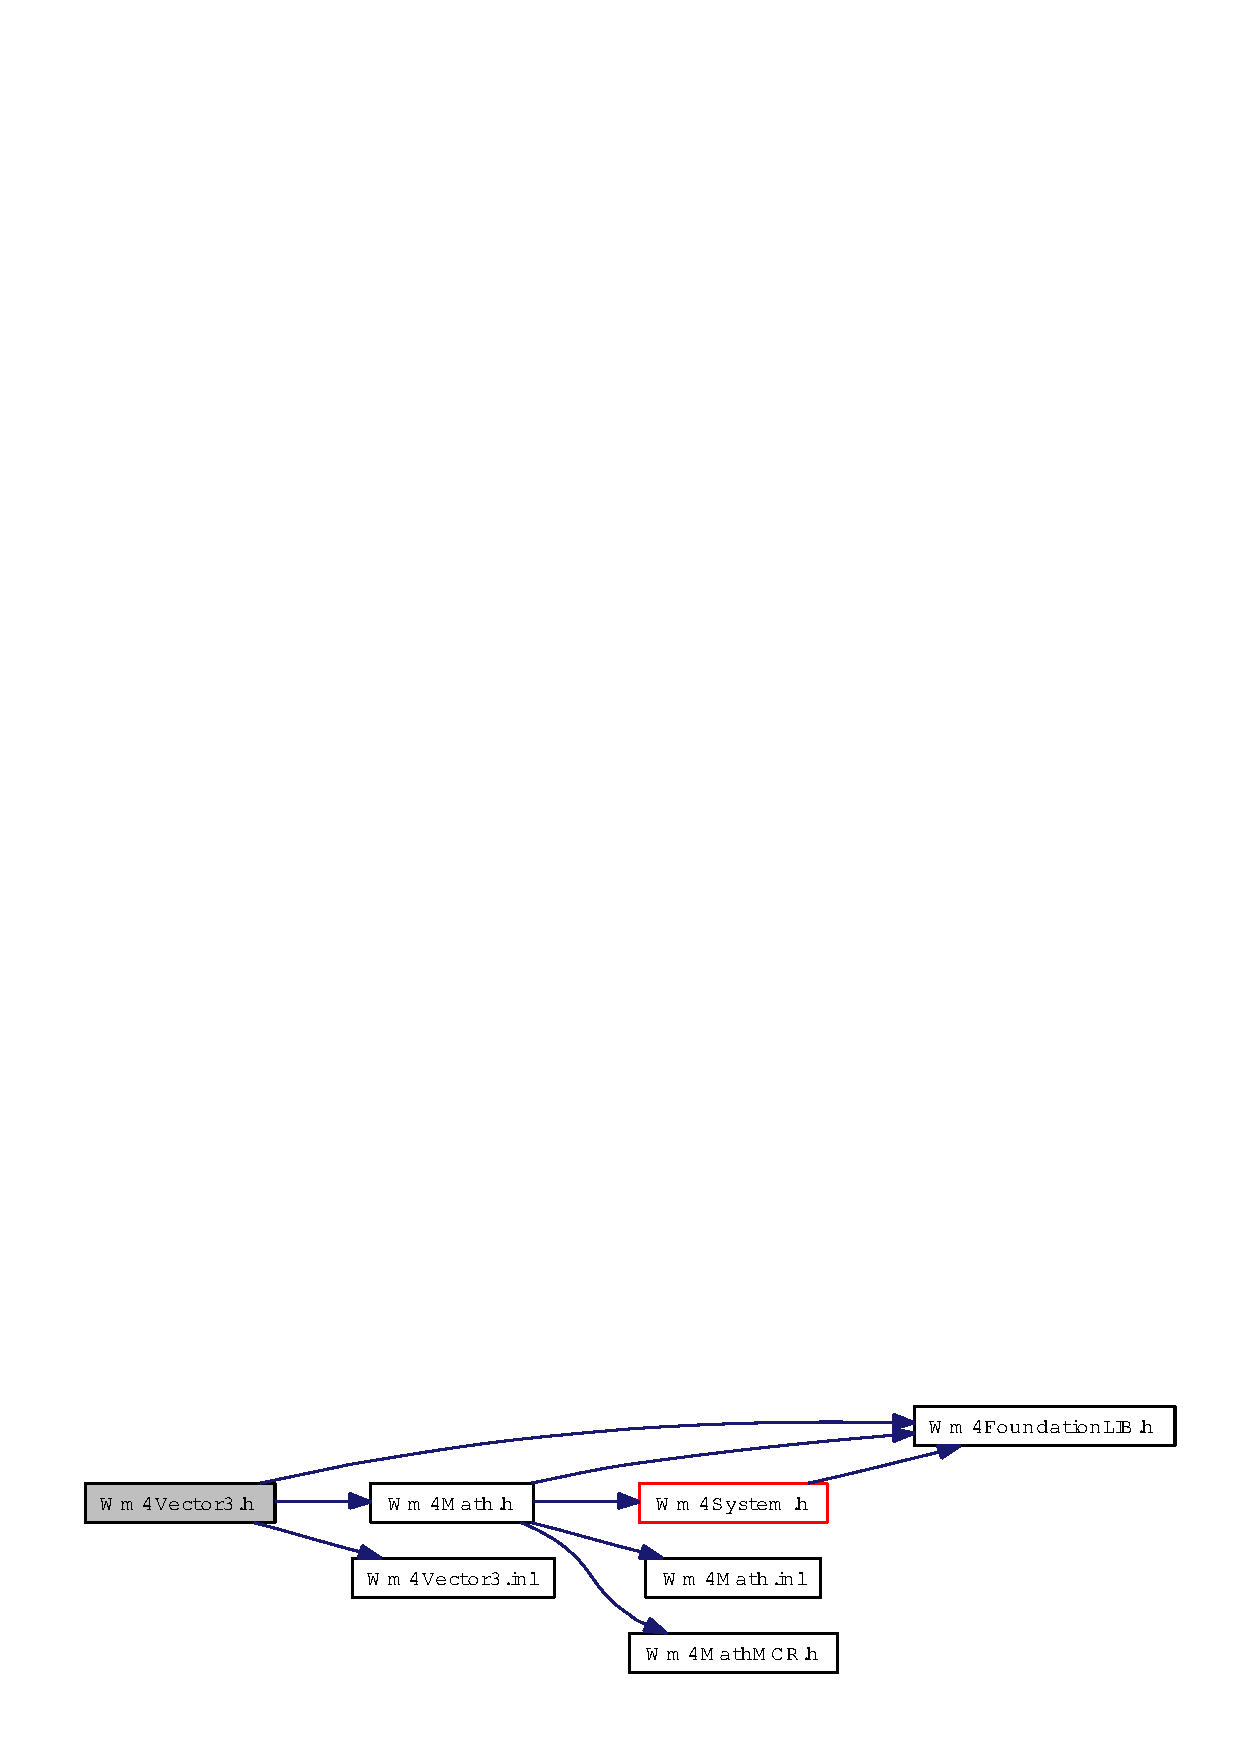
\includegraphics[width=284pt]{Wm4Vector3_8h__incl}
\end{center}
\end{figure}


This graph shows which files directly or indirectly include this file:\begin{figure}[H]
\begin{center}
\leavevmode
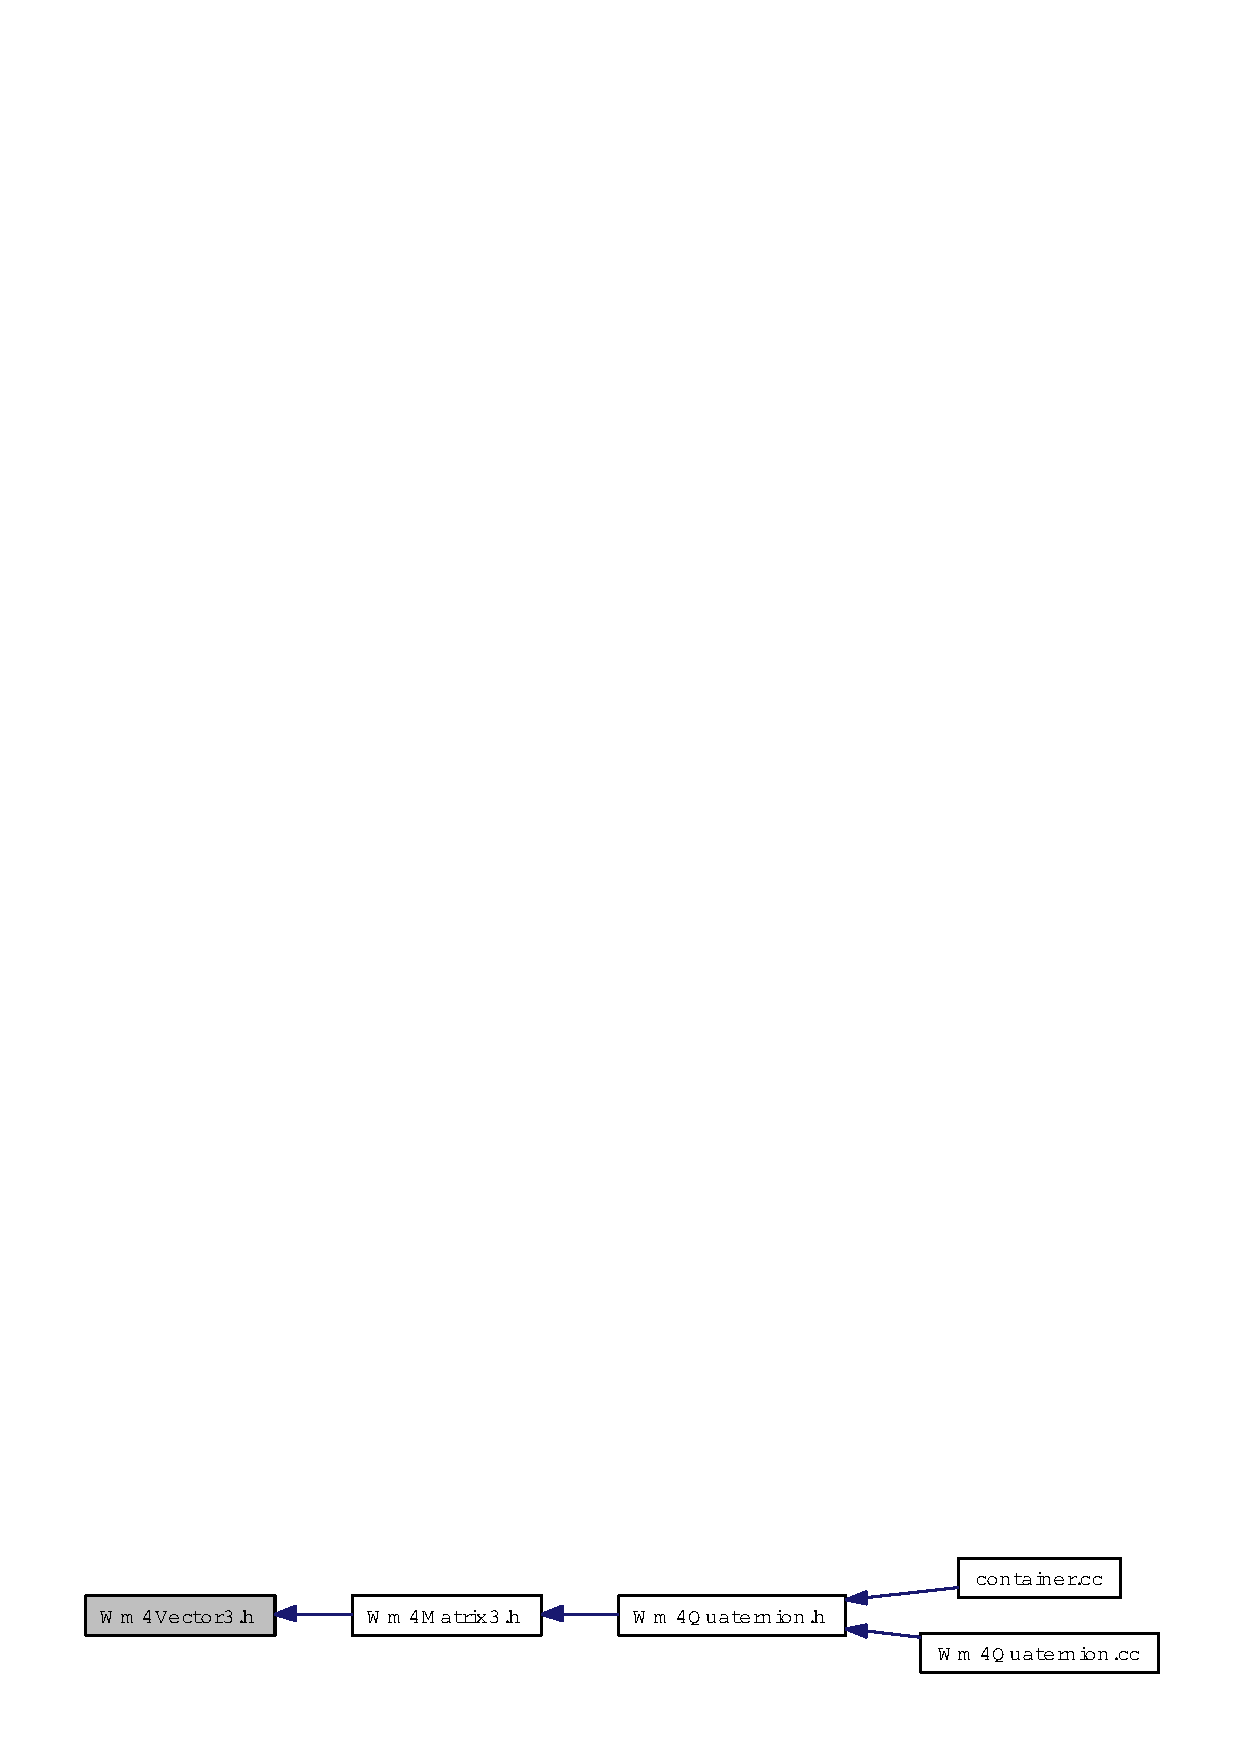
\includegraphics[width=280pt]{Wm4Vector3_8h__dep__incl}
\end{center}
\end{figure}
\subsection*{Namespaces}
\begin{CompactItemize}
\item 
namespace {\bf Wm4}
\end{CompactItemize}
\subsection*{Classes}
\begin{CompactItemize}
\item 
class {\bf Wm4::Vector3$<$ Real $>$}
\end{CompactItemize}
\subsection*{Typedefs}
\begin{CompactItemize}
\item 
typedef Vector3$<$ float $>$ {\bf Wm4::Vector3f}
\item 
typedef Vector3$<$ double $>$ {\bf Wm4::Vector3d}
\end{CompactItemize}
\subsection*{Functions}
\begin{CompactItemize}
\item 
template$<$class Real$>$ Vector3$<$ Real $>$ {\bf Wm4::operator $\ast$} (Real f\-Scalar, const Vector3$<$ Real $>$ \&rk\-V)
\item 
template$<$class Real$>$ std::ostream \& {\bf Wm4::operator$<$$<$} (std::ostream \&rk\-OStr, const Vector3$<$ Real $>$ \&rk\-V)
\end{CompactItemize}
